\chapter{Detalles de Implementación y Experimentos}\label{chapter:implementation}

\section{Detalles de implementaci\'on}

En esta secci\'on se abordar\'an algunos detalles que se tuvieron en cuenta a la hora de implementar este m\'odulo.

\subsection{Modelos}

Primeramente obs\'ervese que el rango de niveles de gris de una imagen se define como $[0,M)$. Por ende al transformar la imagen a una funci\'on de tono de gris utilizando la f\'ormula (1.11) cuando el nivel de gris es 0 el tono de gris es $M$, lo cual contradice que el rango de tono de gris para el modelo LIP es $[0,M)$. Por este motivo tanto para la clase \verb|LIPImage| como \verb|LIPSpace| antes de cambiar la imagen de niveles de gris a tonos de gris y viceversa, esta primero se procesa de tal forma que el menor valor admisible sea un n\'umero cercano a cero, pero mayor que este. En esta implementaci\'on se decidi\'o utilizar el n\'umero $0.0001$. No se opt\'o por otras alternativas como por ejemplo el \'epsilon de la m\'aquina porque al realizar operaciones aritm\'eticas este valor se convert\'ia en cero y por ende no solucionaba el problema planteado. Esto tambi\'en se hizo en la implementaci\'on del modelo PLIP. Para el caso del modelo SLIP no fue necesario pues no se utiliza una funci\'on de cambio a tono de gris y se trabaja directamente con los niveles de gris.

Otro problema que fue necesario resolver es que en el modelo HLIP los niveles de gris de la imagen a transformar deben estar en el rango $(0,M)$. La soluci\'on propuesta fue hacer algo similar al caso anterior, pero solo antes de cambiar la imagen de nivel de gris a tono de gris.

Las implementaciones de todos los modelos tal y como se explic\'o en el cap\'itulo anterior se pueden encontrar en el subm\'odulo ``models'', cada uno en su archivo correspondiente.

\subsection{M\'etricas}

Como se explic\'o en el cap\'itulo exterior se implementaron dos m\'etricas: EMEE y $C_p(p)$. La implementaci\'on de estas m\'etricas se puede encontrar en el subm\'odulo ``metrics''. Este subm\'odulo consta de dos archivos: ``emee.py'' y ``contrast\_pixel''. 

\subsubsection{EMEE}
En el archivo ``emee.py'' se encuentran dos funciones: \verb|emee| y \verb|find_min_max|. La primera devuelve el valor de EMEE de una imagen dada como entrada. Adem\'as recibe como par\'ametros el valor de $\alpha$, las dimensiones de los bloques en los que se desea dividir la imagen y una constante $c$. Esta constante se utiliza para evitar la divisi\'on por $0$ en (1.33). Se suma tanto al numerador como al denominador de las fracciones que aparecen. La constante que se utiliz\'o para calcular los mejores par\'ametros fue $0.5$. Esto tambi\'en para evitar que una divisi\'on por un n\'umero muy cercano a 0 diera un resultado demasiado grande. 

La funci\'on \verb|find_min_max| se utiliza para calcular el menor y mayor valor de intensidad de un bloque. Da como salida una tupla con dicho valores en ese orden y recibe una imagen y 4 enteros: $n_1,n_2,m_1,m_2$, tal que $(n_1,m_1)$ son las coordenadas donde inicia el bloque y; $n_2$ y $m_2$ son la dimensi\'on horizontal y vertical del bloque respectivamente.

\subsubsection{Contraste Promedio}
En el archivo ``contrast\_pixel.py'' se encuentran tres funciones. La primera funci\'on \verb|abs_contrast_2_pixels| se utiliza para calcular el contraste absoluto entre 2 p\'ixeles. Recibe dos \textit{tuplas} de 3 elementos, tal que cada una representa representa un p\'ixel (las coordenadas y el valor de intensidad del p\'ixel), y el valor de $M$.  La segunda funci\'on \verb|contras_pixel| calcula el contraste de un p\'ixel en una imagen; recibe como par\'ametros una \textit{tupla} que representa al p\'ixel, la imagen, el valor de $M$ y un valor $v$ que indica el radio de la vecindad a considerarse. 

La \'ultima funci\'on \verb|contrast_img| da como salida el contraste promedio de un p\'ixel en una imagen, o sea $C_p$. Esta funci\'on recibe como par\'ametros la imagen, el valor de $M$ y el radio de la vecindad que se debe tener en cuenta alrededor de un p\'ixel. Como calcular el contraste para cada p\'ixel de una imagen es un proceso que puede demorar seg\'un el tama\~no de la imagen, se tom\'o la decisi\'on de, para im\'agenes cuya resoluci\'on fuese mayor que $300\times300$, escoger un subconjunto de p\'ixeles. El criterio para escoger dichos p\'ixeles fue el siguiente:

\begin{enumerate}
	\item Iniciar desde la posici\'on $(0,0)$
	\item Si se analiz\'o el pixel en la posici\'on $(i,j)$ el pr\'oximo p\'ixel a analizar es el p\'ixel $(i,j+3)$
	\item Una vez terminada de analizar una fila $i$ la pr\'oxima fila a analizar es la fila $i+3$.
\end{enumerate}

El radio de la vecindad que se tom\'o para calcular el contraste de cada p\'ixel fue de 2. Al comparar ambas formas se pudo comprobar que, para im\'agenes con una resoluci\'on grande, la forma propuesta, reduce considerablemente el tiempo de ejecuci\'on, afectando en una cantidad despreciable el resultado final.

\subsection{Algoritmos}

La implementaci\'on de los algoritmos explicados en el cap\'itulo anterior se encuentra en el subm\'odulo ``algorithms''. Este subm\'odulo se compone de tres archivos: ``edge\_detection'', ``unsharp\_masking'' y ``affine\_transform.py''.

\subsubsection{Detecci\'on de Bordes}

El archivo ``edge\_detection'' tiene implementadas dos funciones: \verb|edge_detection| y \verb|space_edge_detection|. La primera recibe como par\'ametros una imagen y un filtro y da como salida el resultado de aplicarle el filtro a la imagen. 

La segunda funci\'on, adem\'as de recibir estos mismos par\'ametros, recibe una instancia de tipo \verb|LogSpace|. Este se utiliza para indicar el modelo que se desea a utilizar. El funcionamiento es sencillo: se transforma la imagen al isomorfismo utilizando primeramente la funci\'on de cambio a tonos de gris y luego la funci\'on del isomorfismo, se aplica el filtro a la imagen transformada y se regresa este resultado al espacio original utilizando primero la inversa de la funci\'on del isomorfismo y luego la funci\'on de cambio a niveles de gris. Recu\'erdese que los modelos que no utilizan funciones de cambio, en su implementaci\'on, dan como salida la misma imagen dada de entrada.

\subsubsection{Unsharp Masking}

El archivo ``unsharp\_masking.py'' consta de dos funciones: \verb|unsharp_masking| y \verb|space_unsharp_masking|. La primera recibe como par\'ametros una imagen, un filtro y un \textit{string} que puede ser: \verb|``+''| o \verb|``-''|. La salida de esta funci\'on es el resultado de utilizar el filtro para detectar los bordes de la imagen y fusionar la imagen original y la imagen de bordes utilizando la suma (\verb|``+''|) o la resta (\verb|``-''|) lineal. 

La segunda funci\'on, adem\'as de recibir estos mismos par\'ametros, recibe una instancia de tipo \verb|LogSpace|. Este algoritmo primero transforma la imagen al isomorfismo utilizando primeramente la funci\'on de cambio a tonos de gris y luego la funci\'on del isomorfismo, se aplica el filtro dado y luego seg\'un el operador especificado, a la imagen original se le suma o se le resta la imagen de bordes. Finalmente se utilizan la inversa del isomorfismo y la imagen de cambio a niveles de gris para regresar al espacio original. El permitir que la que fusi\'on, adem\'as de con la suma se haga con la resta, se tom\'o como decisi\'on despu\'es de que uno de los modelos mostr\'o buenos resultados utilizando la resta en lugar de la suma. 

\subsubsection{Transformaci\'on Af\'in}

El archivo ``affine\_transform.py'' contiene a \verb|space_affine_transform| como \'unica funci\'on definida. Recibe como par\'ametros una imagen y los extremos del intervalo en el cual se va a realizar la transformaci\'on. 

Esta funci\'on da como salida la transformaci\'on af\'in explicada en el cap\'itulo anterior utilizando las operaciones aritm\'eticas de un modelo espec\'ifico. Recibe como par\'ametros una imagen, los extremos del intervalo en el cual se va a realizar la transformaci\'on y una instancia de tipo \verb|LogSpace|. Este \'ultimo par\'ametro se utiliza para indicar con que modelo se quiere realizar la transformaci\'on. Los extremos del intervalo de entrada deben ser los del modelo utilizado para obtener los mejores resultados.

\section{Experimentos}
Para los experimentos que a continuaci\'on se muestran se utilizaron im\'agenes en escala de gris de 8 bits, o sea que los valores de intensidades de los pixeles eran n\'umeros enteros en el intervalo $[0,255]$. Aqu\'i es importante aclarar que los modelos trabajan y dan resultados utilizando n\'umeros de tipo \textit{float64}. Para el mostrado y guardado de las im\'agenes \verb|skimage| primero rescala las im\'agens a n\'umeros flotantes entre $[0,1]$ haciendo \textit{stretching} utilizando como extremos los valores de menor y mayor intensidad presentes en la imagen. Luego esta se lleva a la escala de enteros de 8 bits para mostrar y guardar la imagen~\cite{image_data_types_and_what_they_mean}.

\subsection{Curvas de los isomorfismos}
Lo primero que se muestra son las curvas de los diferentes isomorfismos, iniciando por los no parametrizados que se muestran en la Fig 3.1. Para los isomorfismos LIP y PSLIP se muestra adem\'as los puntos respectivos a los valores: 0 (rojo), 128 (naranja) y 255(amarillo). Para el caso de HLIP se muestran los puntos para los valores: 1 (rojo), 128 (naranja) y 255 (amarillo). Para el caso del modelo SLIP se muestran los puntos para los valores: -255 (morado) -128(verde) 0 (rojo), 128 (naranja) y 255(amarillo).

\begin{figure}
	\begin{center}
		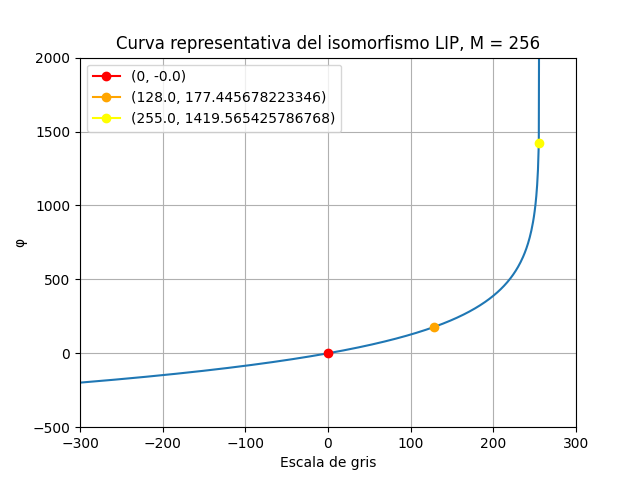
\includegraphics[width=5.5 cm]{images/clasics_curves/lip_curve.png}
		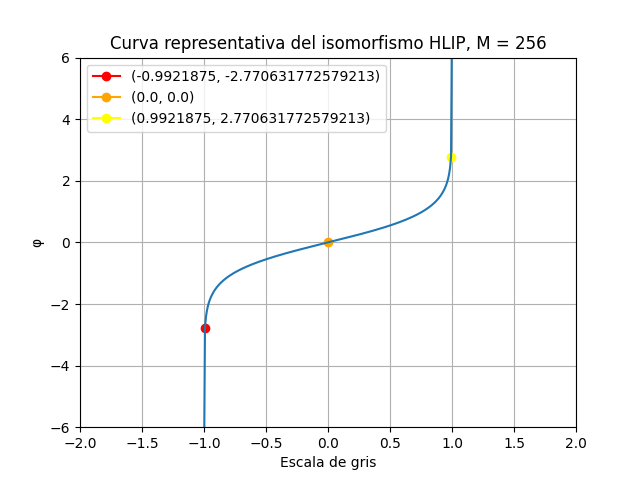
\includegraphics[width=5.5 cm]{images/clasics_curves/hlip_curve.png}
		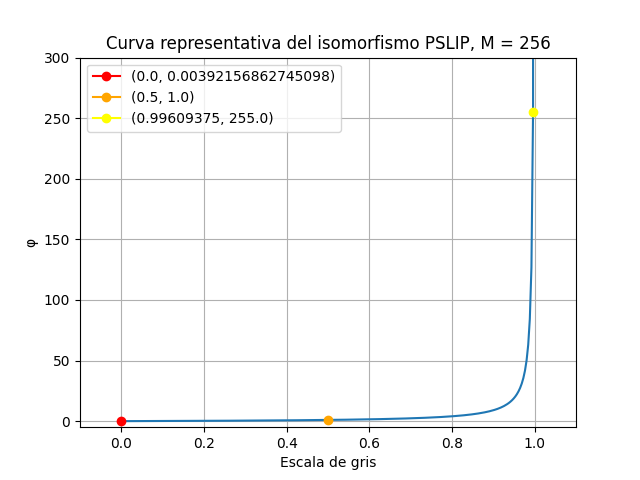
\includegraphics[width=5.5 cm]{images/clasics_curves/pslip_curve.png}
		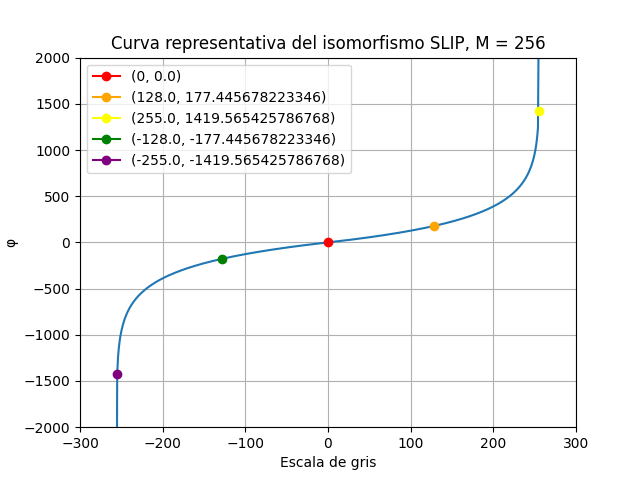
\includegraphics[width=5.5 cm]{images/clasics_curves/slip_curve.png}
		\caption{Curvas representativas de los modelos no parametrizados}
	\end{center}
\end{figure}

En las Fig 3.2 y Fig 3.3 se pueden observar varias curvas del modelo PLIP y PPSLIP utilizando diferentes valores de $\lambda(M)$. En ambos modelos se puede apreciar la tendencia a la linealidad a medida que el valor de $\lambda(M)$ aumenta. Obse\'ervese que los puntos correspondiente a 0 (rojo), 128 (naranja) y 255 (amarillo) se van acercando a una l\'inea recta. Tambi\'en se muestra que los nuevos valores que aparecen siguen manteniendo la estructura logar\'itmica.

\begin{figure}
	\begin{center}
		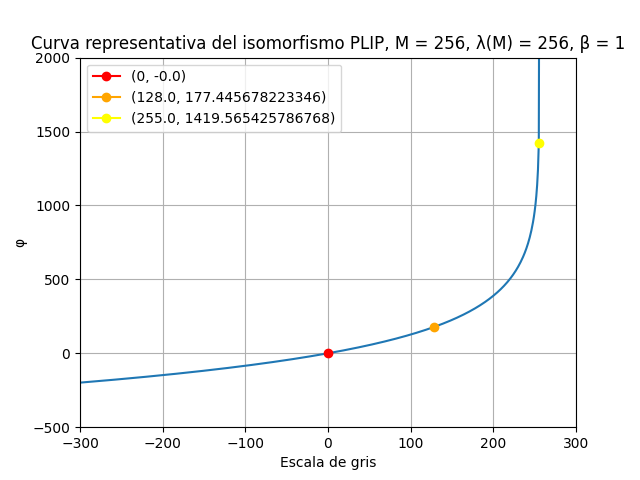
\includegraphics[width=5.5 cm]{images/plip_curves/plip_curve_256.png}
		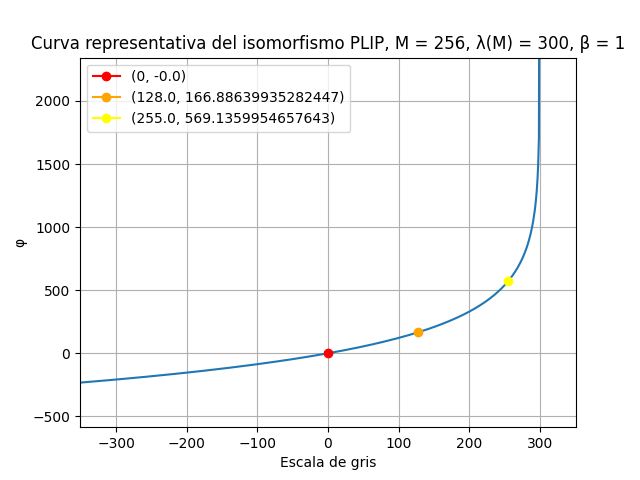
\includegraphics[width=5.5 cm]{images/plip_curves/plip_curve_300.png}
		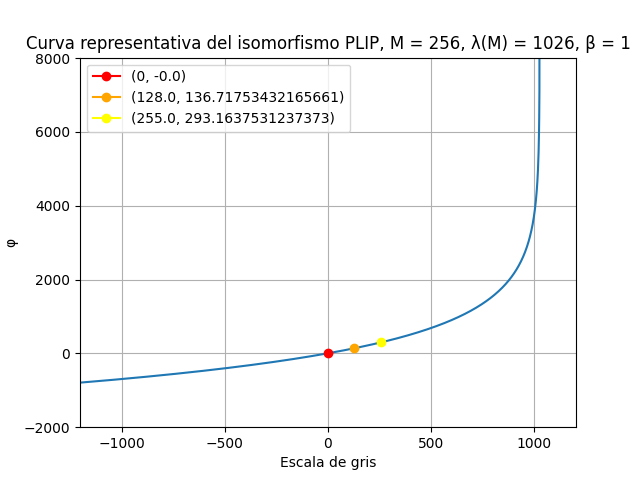
\includegraphics[width=5.5 cm]{images/plip_curves/plip_curve_1026.png}
		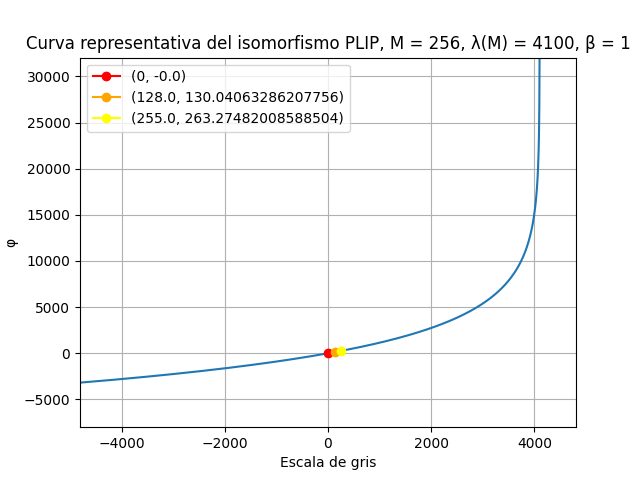
\includegraphics[width=5.5 cm]{images/plip_curves/plip_curve_4100.png}
		\caption{Curvas representativas del modelo PLIP con diferentes valores de $\lambda(M)$}
	\end{center}
\end{figure}

\begin{figure}
	\begin{center}
		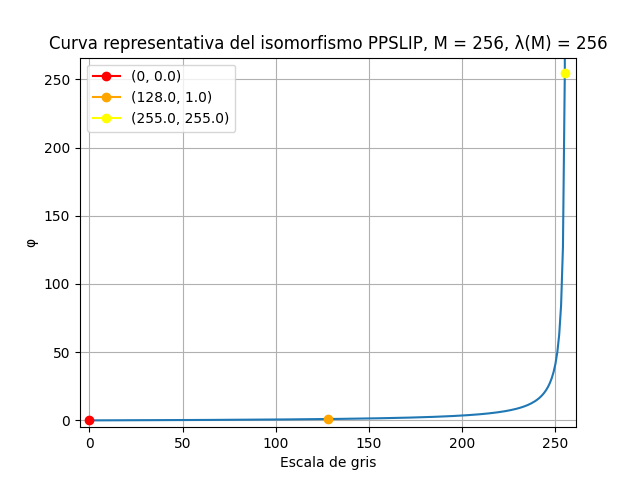
\includegraphics[width=5.5 cm]{images/ppslip_curves/ppslip_curve_256.png}
		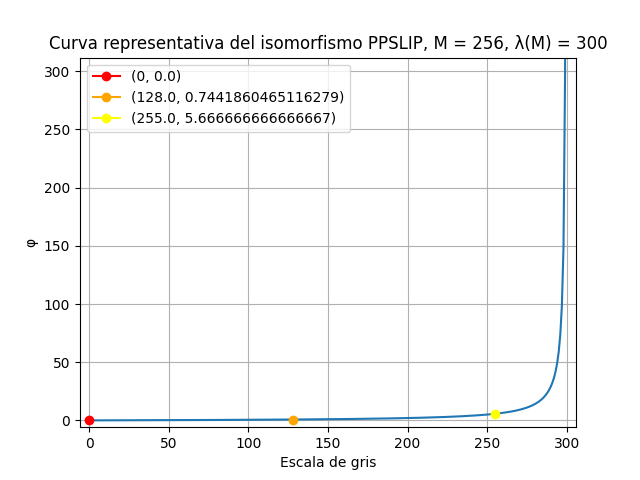
\includegraphics[width=5.5 cm]{images/ppslip_curves/ppslip_curve_300.png}
		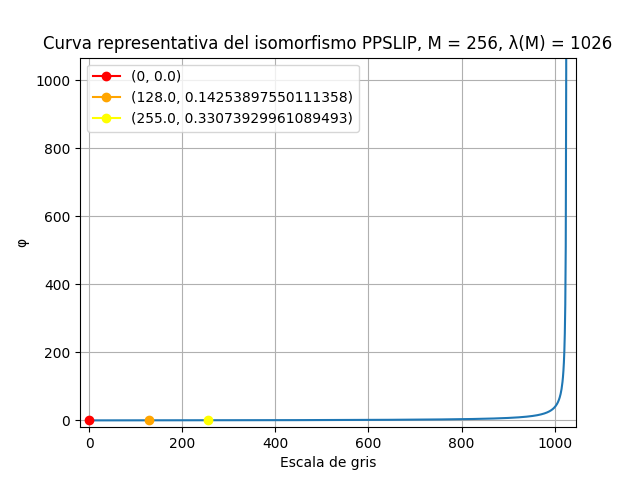
\includegraphics[width=5.5 cm]{images/ppslip_curves/ppslip_curve_1026.png}
		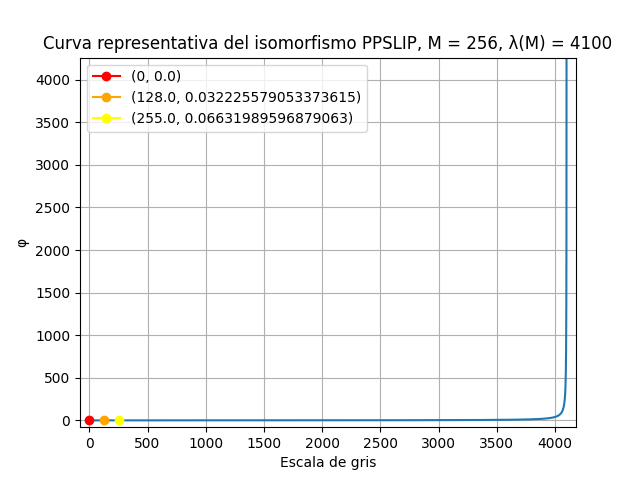
\includegraphics[width=5.5 cm]{images/ppslip_curves/ppslip_curve_4100.png}
		\caption{Curvas representativas del modelo PPSLIP con diferentes valores de $\lambda(M)$}
	\end{center}
\end{figure}

\subsection{Suma de im\'agenes}

Una de las formas m\'as utilizadas para la fusi\'on de im\'agenes es la suma de las mismas. Para los experimentos que se muestran a continuaci\'on se utilizar\'an las im\'agenes: Playa, Patineta, Monta\~na e Insecto que se muestran en la Fig 3.4.

\begin{figure}
	\begin{center}
		\subfigure[Playa]{
		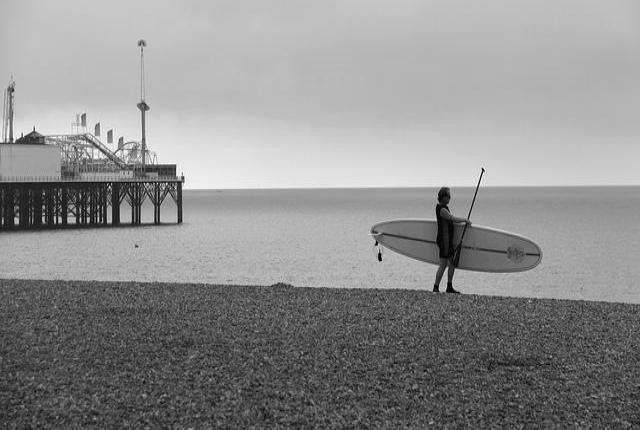
\includegraphics[width=5.5 cm]{images/originals/playa.jpg}}
		\subfigure[Patineta]{
			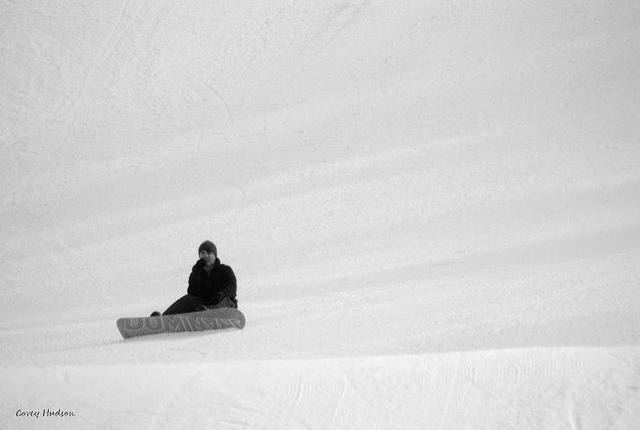
\includegraphics[width=5.5 cm]{images/originals/patineta.jpg}}
		\subfigure[Monta\~na]{
			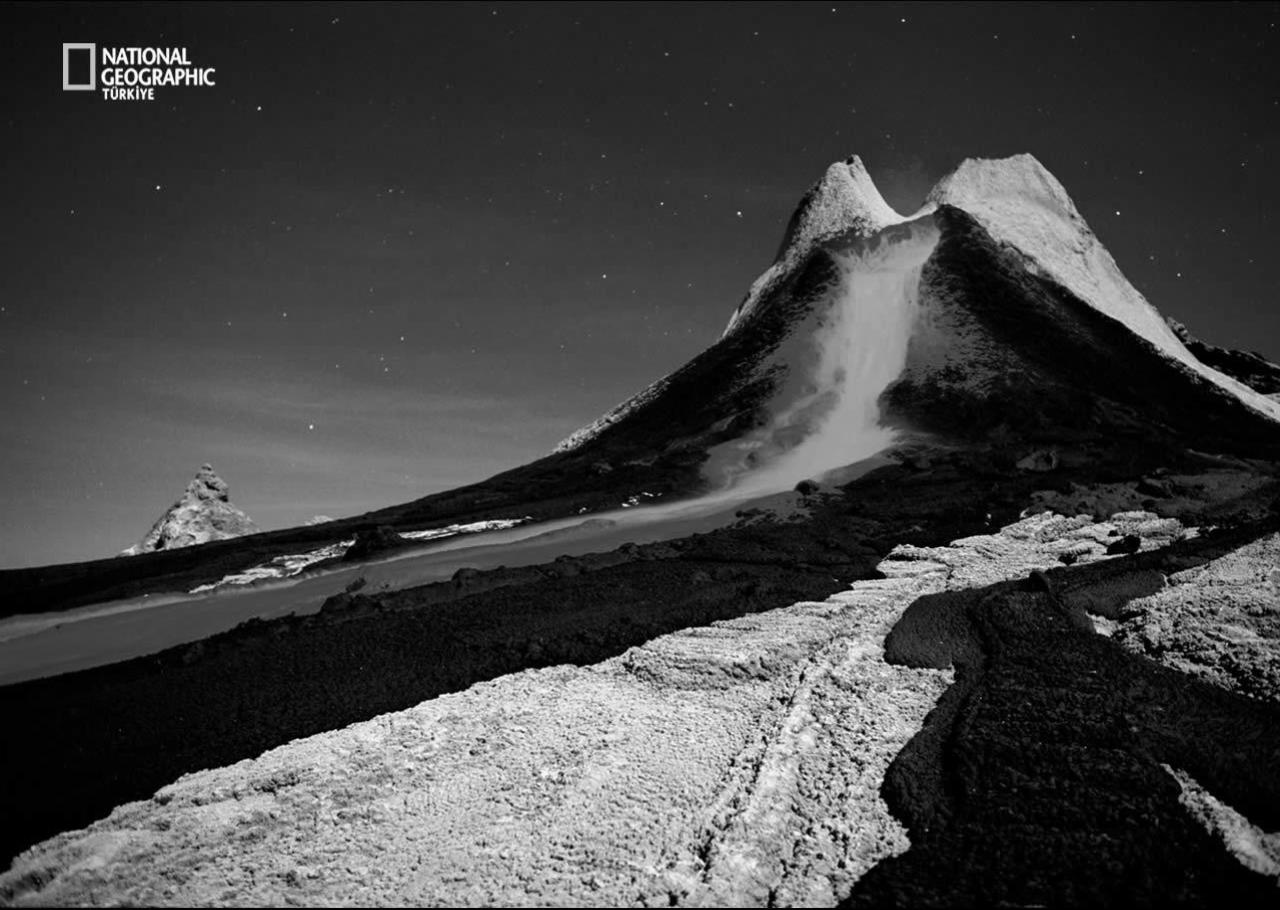
\includegraphics[width=5.5 cm]{images/originals/montania.jpg}}
		\subfigure[Insecto]{
			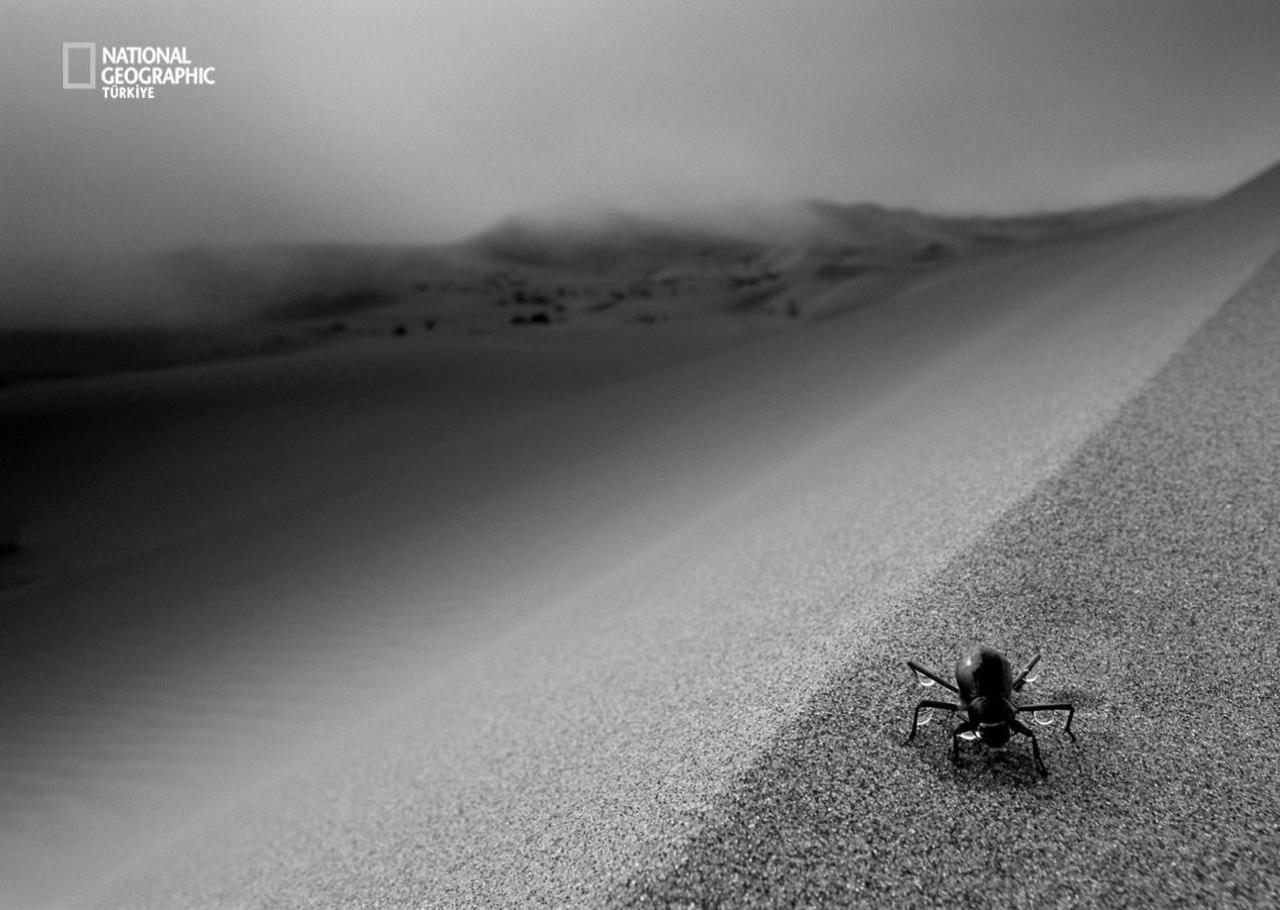
\includegraphics[width=5.5 cm]{images/originals/insecto.jpg}}
		\caption{Im\'agenes para los experimentos de suma}
	\end{center}
\end{figure}

\begin{figure}
	\begin{center}
		\subfigure[Lineal $C_p=3.49$]{
			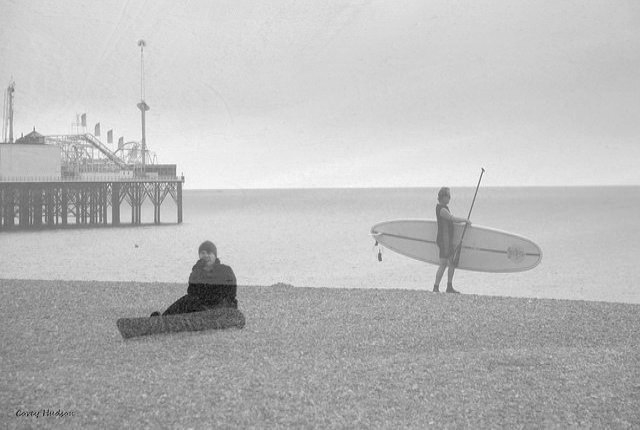
\includegraphics[width=5.5 cm]{images/sums/p y p/sab.png}}
		\subfigure[LIP $C_p=5.71$]{
			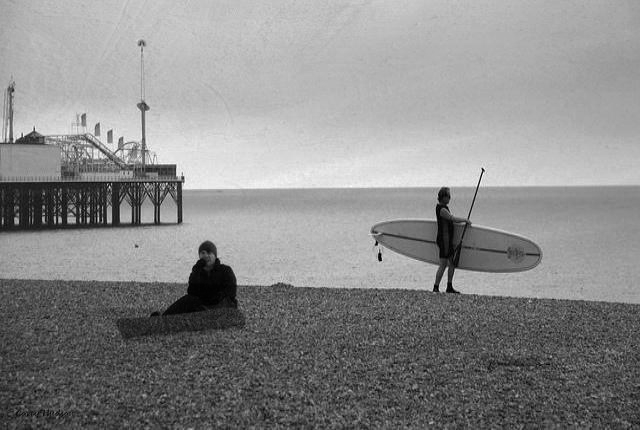
\includegraphics[width=5.5 cm]{images/sums/p y p/jsab.png}}
		\subfigure[HLIP $C_p=4.96$]{
			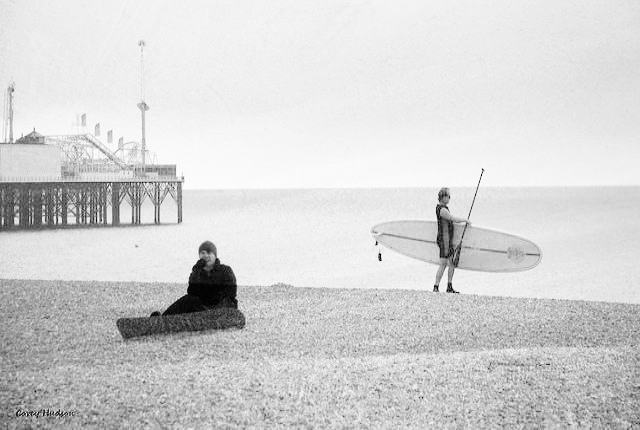
\includegraphics[width=5.5 cm]{images/sums/p y p/hsab.png}}
		\subfigure[PSLIP $C_p=1.39$]{
			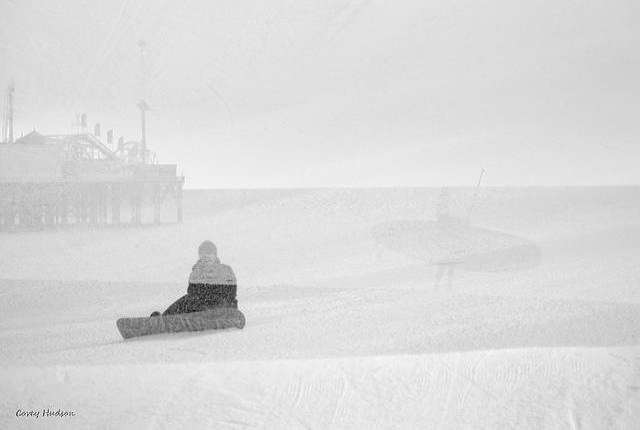
\includegraphics[width=5.5 cm]{images/sums/p y p/pssab.png}}
		\subfigure[SLIP $C_p=1.45$]{
			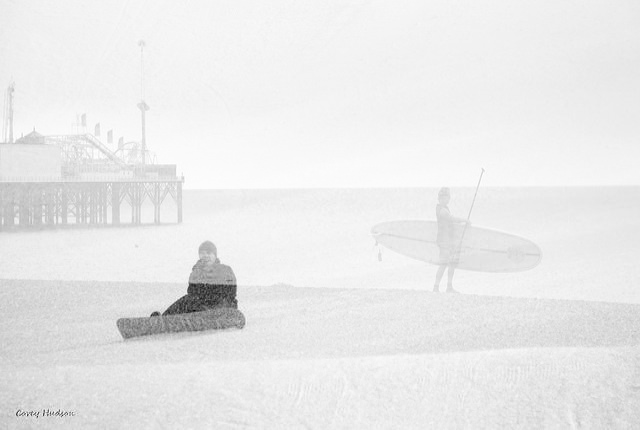
\includegraphics[width=5.5 cm]{images/sums/p y p/ssab.png}}
		\subfigure[PLIP $C_p=5.71$]{
			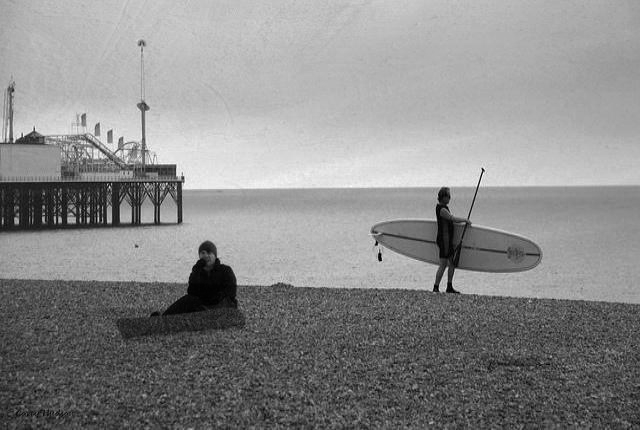
\includegraphics[width=5.5 cm]{images/sums/p y p/psab.png}}
		\subfigure[PPSLIP $C_p=3.35$]{
			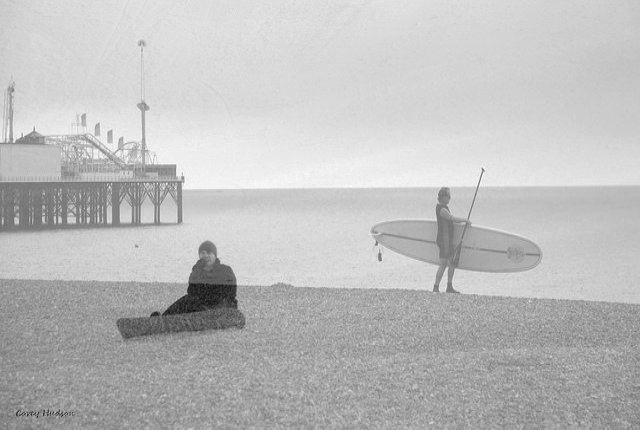
\includegraphics[width=5.5 cm]{images/sums/p y p/ppssab.png}}
		\caption{Suma de Playa y Patineta utilizando los diferentes modelos}
	\end{center}
\end{figure}

\begin{figure}
	\begin{center}
		\subfigure[Lineal $C_p=3.15$]{
			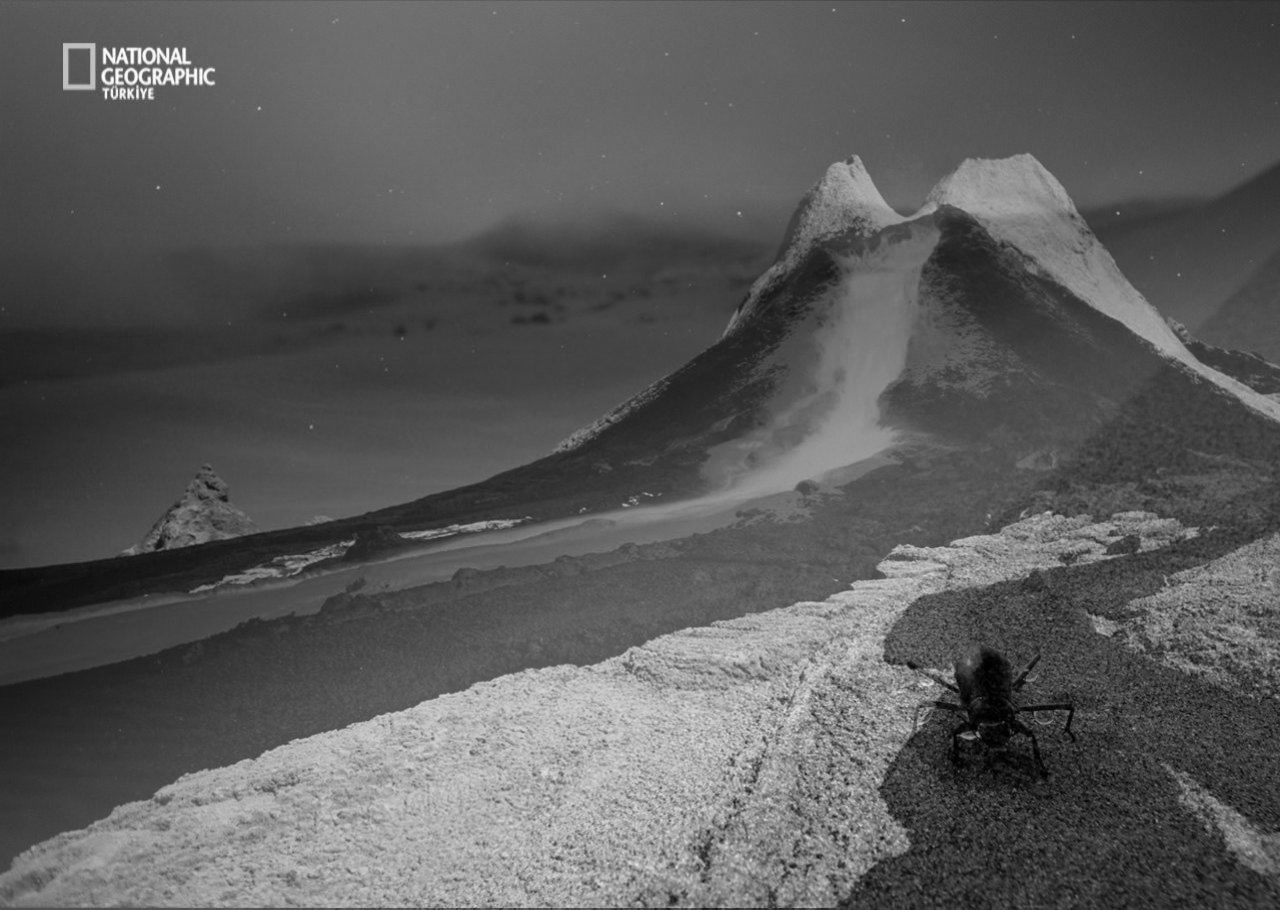
\includegraphics[width=5.5 cm]{images/sums/m y i/scd.png}}
		\subfigure[LIP $C_p=2.77$]{
			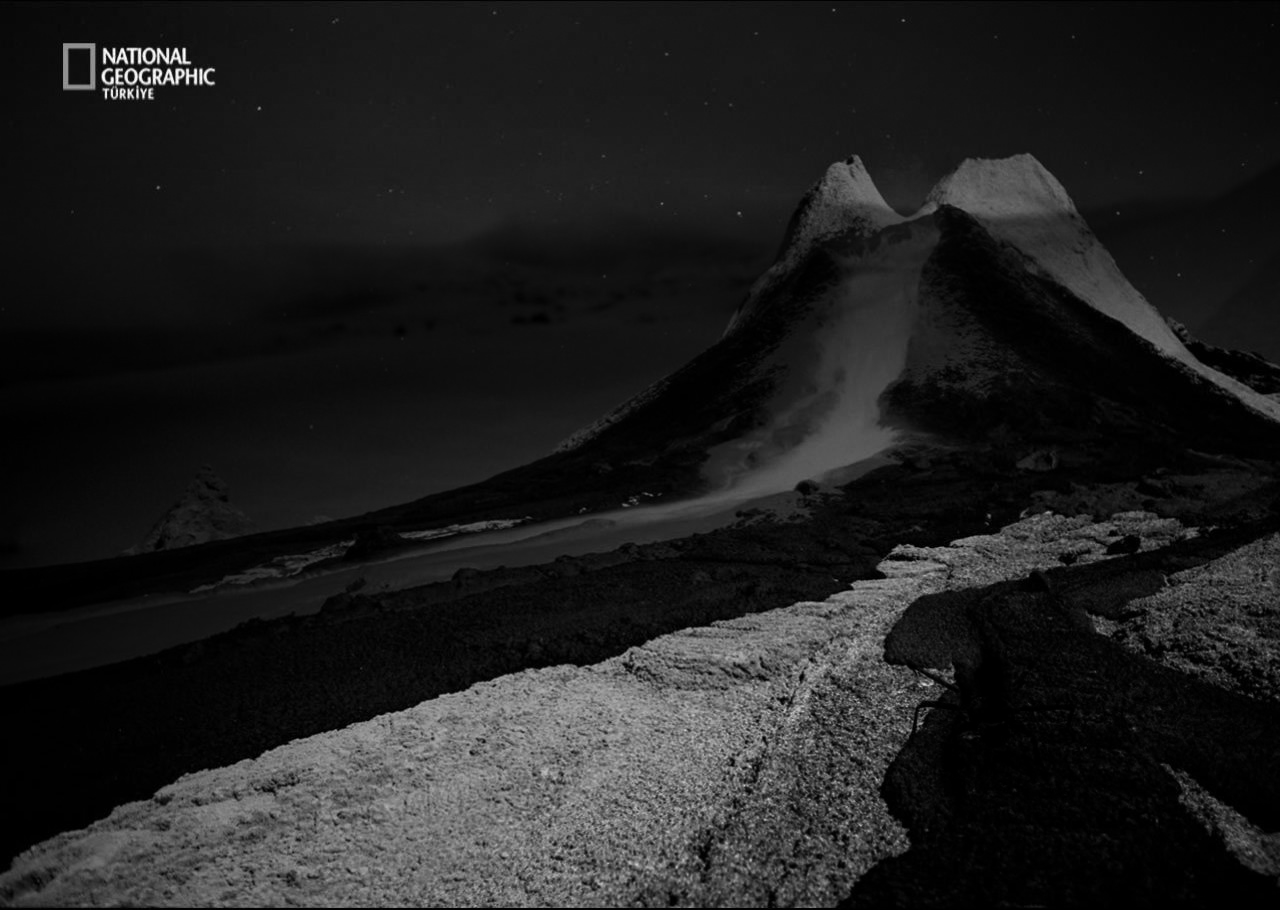
\includegraphics[width=5.5 cm]{images/sums/m y i/jscd.png}}
		\subfigure[HLIP $C_p=4.53$]{
			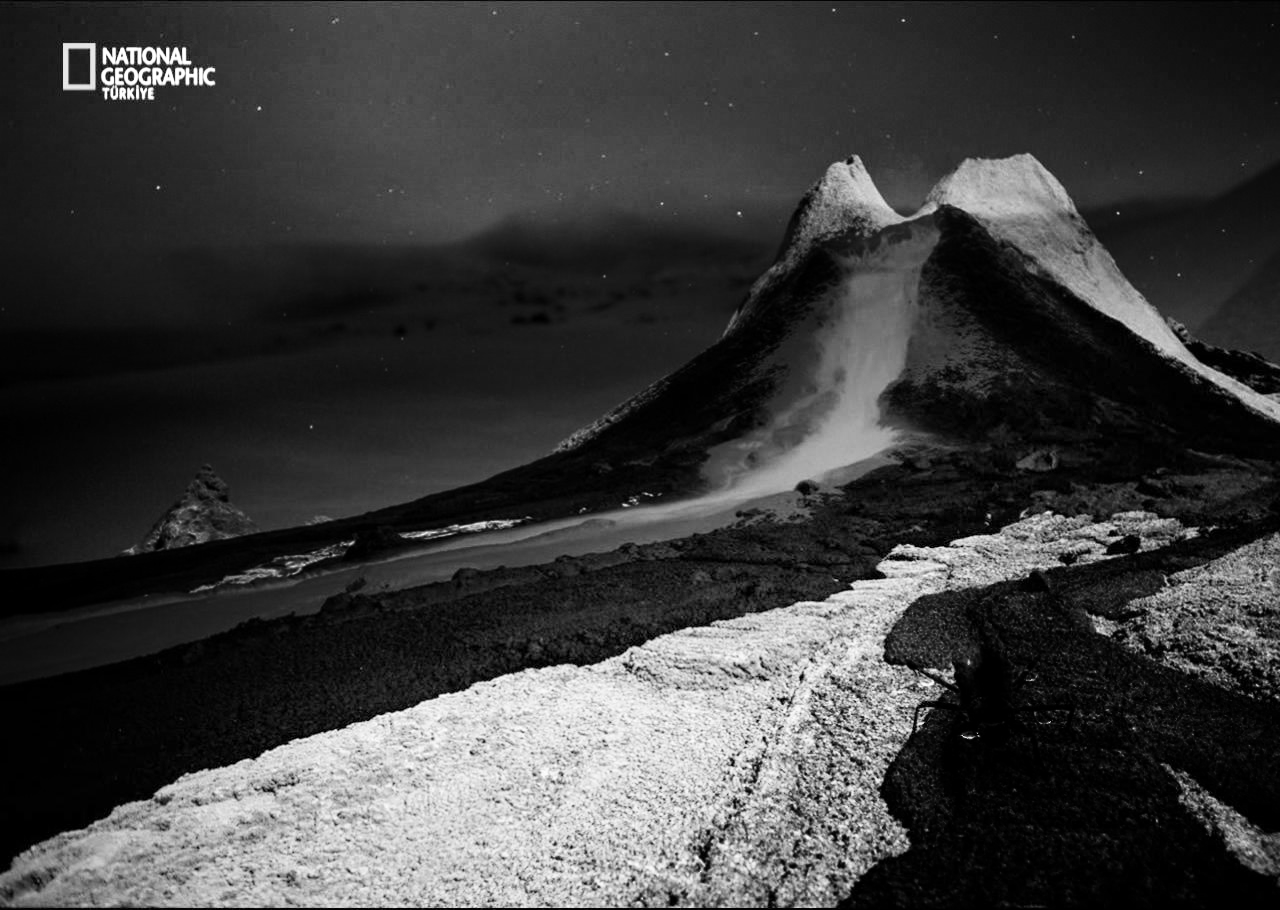
\includegraphics[width=5.5 cm]{images/sums/m y i/hscd.png}}
		\subfigure[PSLIP $C_p=3.47$]{
			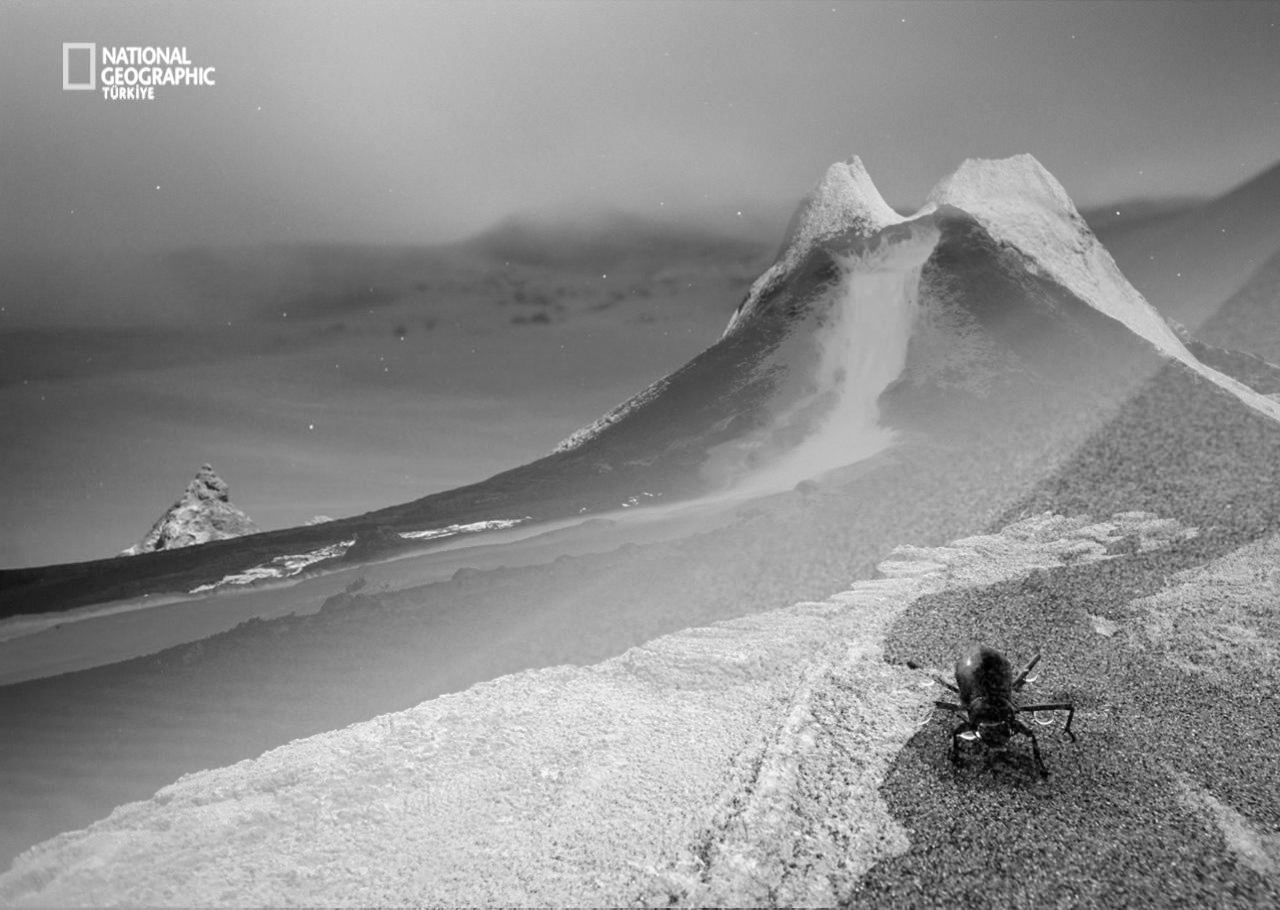
\includegraphics[width=5.5 cm]{images/sums/m y i/psscd.png}}
		\subfigure[SLIP $C_p=3.65$]{
			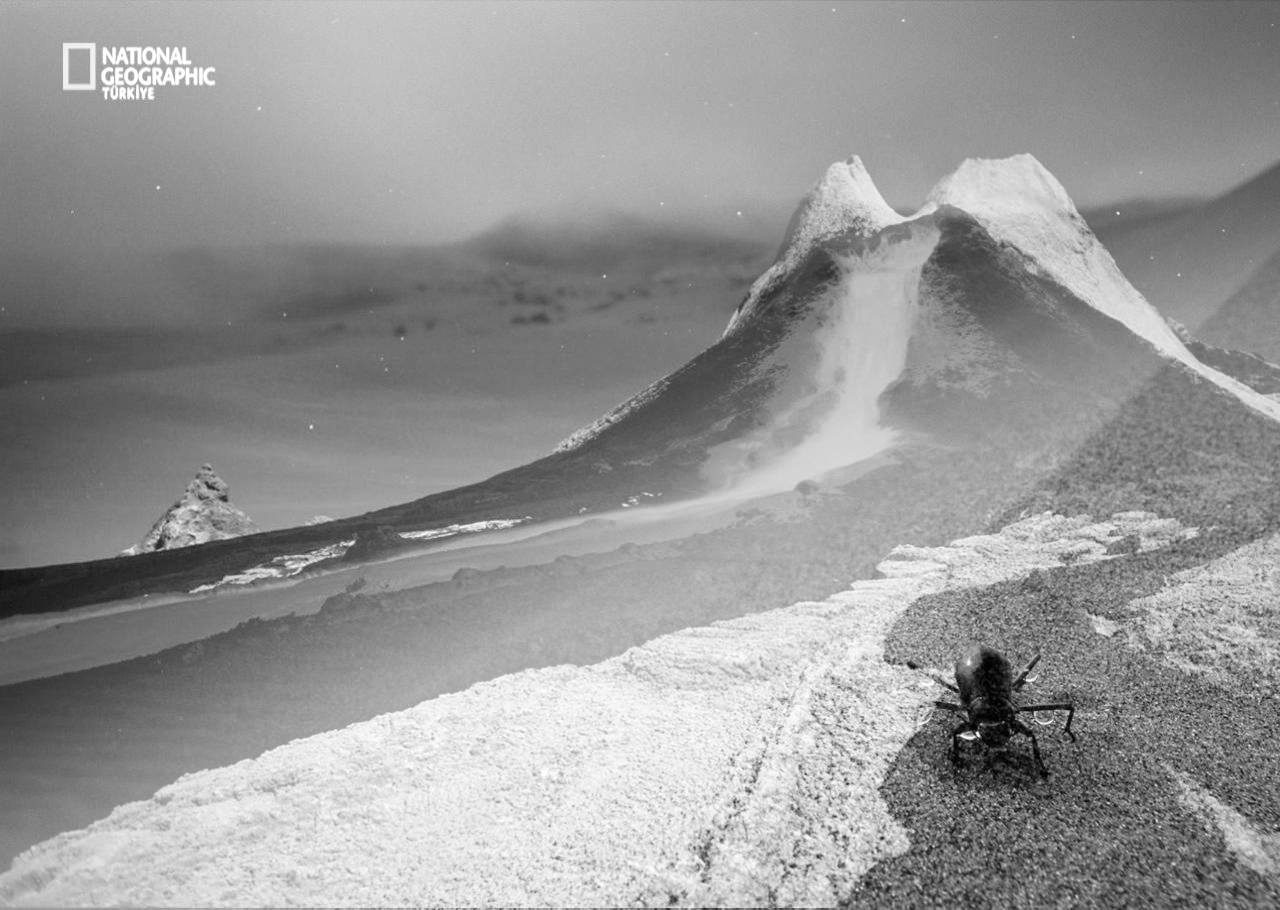
\includegraphics[width=5.5 cm]{images/sums/m y i/sscd.png}}
		\subfigure[PLIP $C_p=3.13$]{
			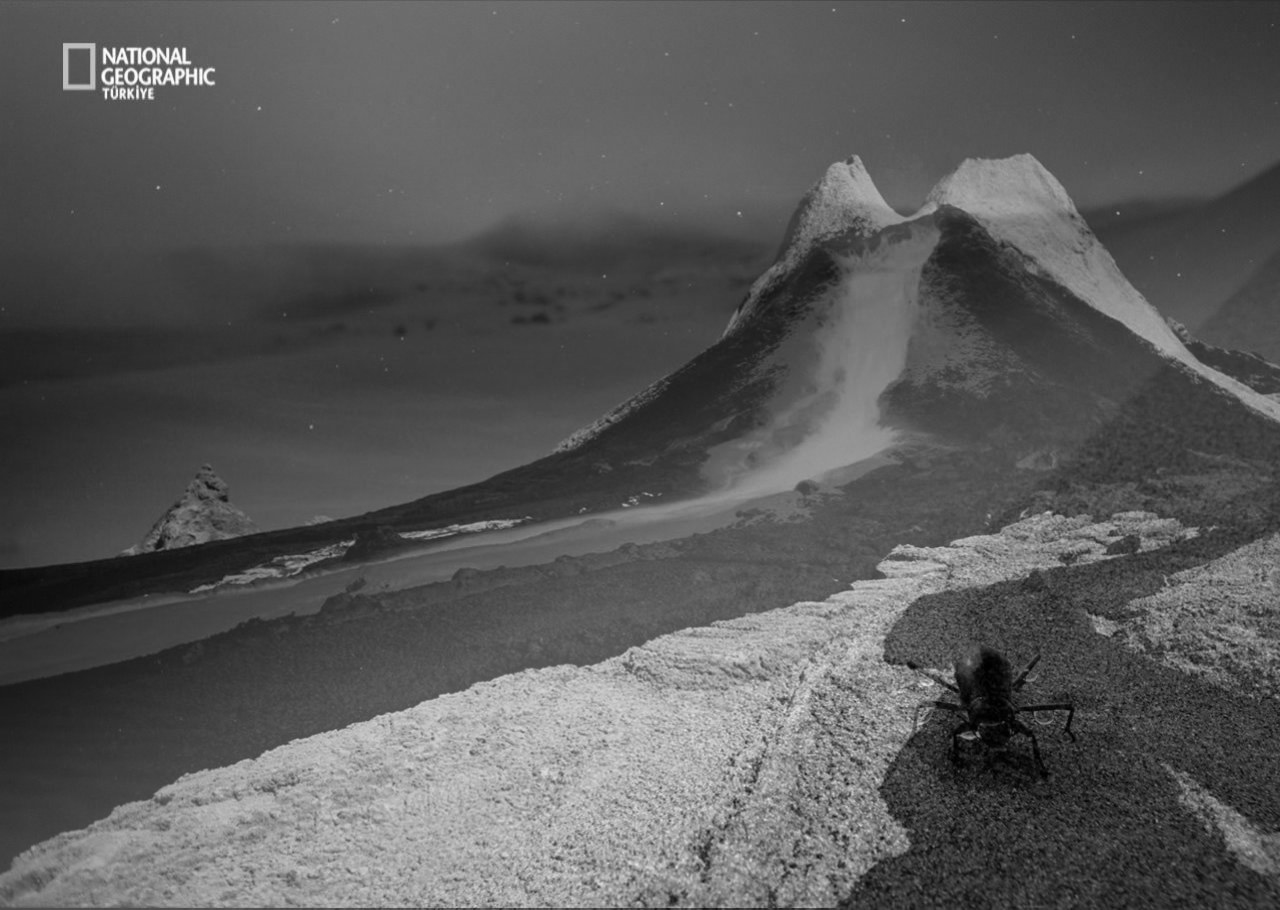
\includegraphics[width=5.5 cm]{images/sums/m y i/pscd.png}}
		\subfigure[PPSLIP $C_p=3.47$]{
			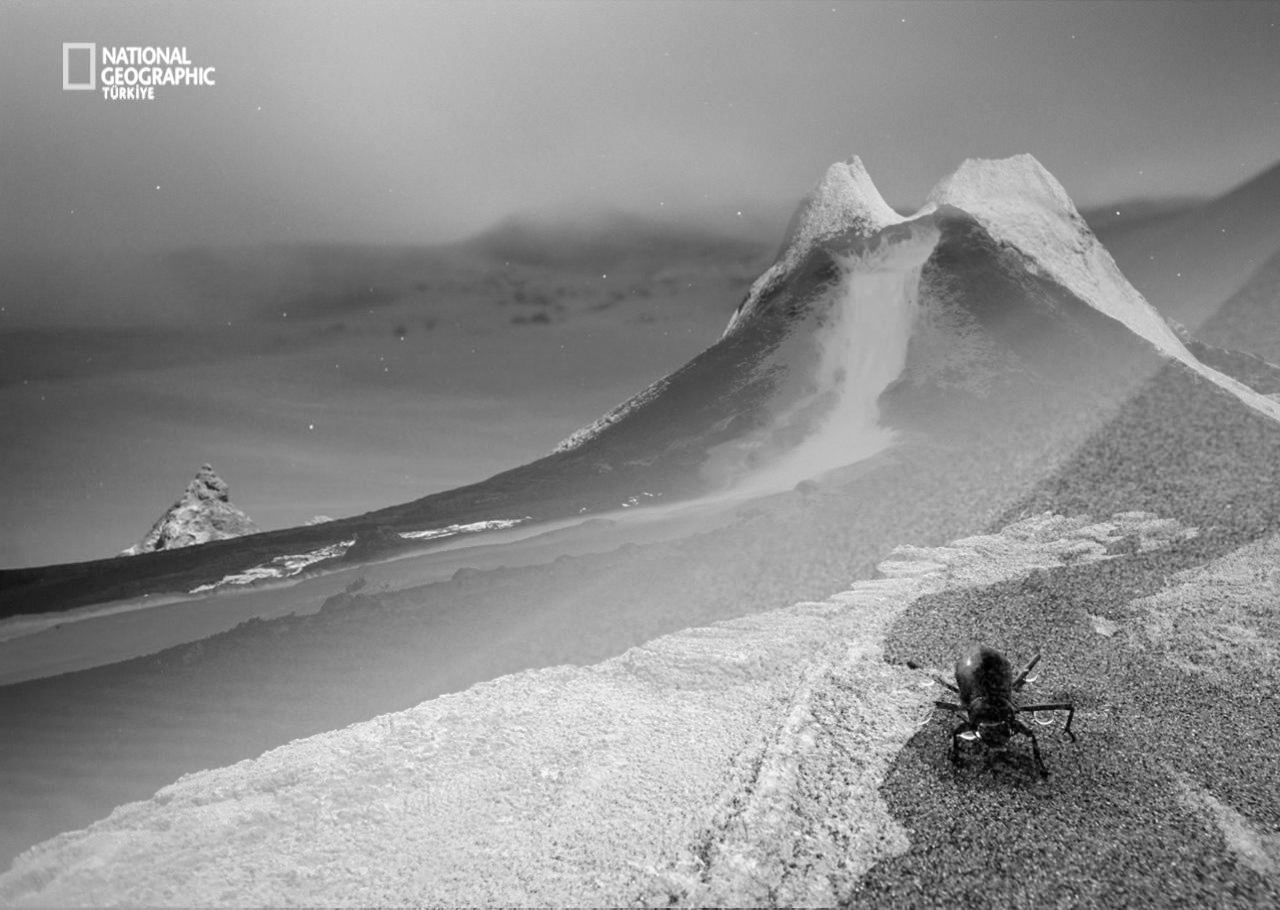
\includegraphics[width=5.5 cm]{images/sums/m y i/ppsscd.png}}
		\caption{Suma de Monta\~na e Insecto utilizando los diferentes modelos}
	\end{center}
\end{figure}

En la Fig 3.5 se muestra la de la imagen  ``Playa'' y la imagen ''Patineta'' utilizando los diferentes modelos. En esta figura se puede apreciar que el mejor valor de contraste promedio $C_p$ es el del modelo LIP. Adem\'as se puede apreciar que las im\'agenes dada por los modelos SLIP y PSLIP son im\'agenes claras mientras que para el modelo LIP esta es m\'as oscura. Esto es l\'ogico debido a que en el modelo LIP, se invierte la escala de gris mientras que en los dos antes mencionados esto no ocurre. El modelo HLIP muestra un comportamiento balanceado, como era de esperarse debido a su simetr\'ia. Dado que el modelo LIP es que el mejor resultado arroja, en consecuencia el modelo PLIP se comporta como este, mientras que al dar, el modelo PSLIP un valor de contraste peor al del modelo lineal, es l\'ogico que este tienda a la linealidad.

Para determinar los par\'ametros de $\gamma(M)$ y $\mu(M)$ en el modelo PLIP, se aplic\'o el cambio a tonos de gris utilizando el valor de $M=256$. Luego se prob\'o la suma con diferentes valores de $\gamma(M)$ (256, 300, 1026 y 4100) y por cada uno se probaron varios valores de $\mu(M)$ para cambiar a niveles de grises. Para determinar el mejor valor de $\mu(M)$ para cada $\gamma(M)$ se utiliz\'o la m\'etrica EMEE. Luego se calcul\'o el valor de $C_p$ por cada pareja y el mejor valor se obtuvo para $\mu(M)=256$ y $\gamma(M)=256$. Para determinar el mejor valor de $\gamma(M)$ para el modelo PPSLIP se realiz\'o la operaci\'on de suma utilizando varios par\'ametros y se determin\'o el mejor utilizando el valor de $C_p$, el resultado fue de $\gamma(M)=4100$. 

En la figura 3.6 se puede observar otro ejemplo de la suma. En este caso el modelo LIP arroja una imagen muy oscura, mientras que el modelo lineal ofrece una m\'as clara. M\'as claras a\'un y con mejor valor de $C_p$ son las im\'agenes obtenidas por los modelos PSLIP y SLIPo. Se vuelve a apreciar el balance en el modelo HLIP, dando una imagen donde se combinan en gran medida los negros y los blancos, dando el mejor valor de $C_p$. En esta caso el modelo PLIP tendi\'o a la linealidad para lograr un mejor valor de $C_p$, mientras que por su parte el modelo PPSLIP se asemej\'o al modelo PPSLIP.

Con estos experimentos ya se puede ir percatando lo que te\'oricamente se esperaba: la sensibilidad del modelo PLIP hacia los niveles de gris m\'as oscuros, la sensibilidad de los modelos PSLIP y SLIP hacia los niveles de gris m\'as claros y el balance que entre ambos que supone el modelo HLIP dado su car\'acter sim\'etrico. Aqu\'i aclarar que el modelo SLIP, aunque tambi\'en es sim\'etrico, una imagen trasformada a este modelo no se expande por toda la escala de gris del modelo como si ocurre en el HLIP, a no ser que se haga eso manualmente. Tambi\'en se puede apreciar como los modelos parametrizados utilizan los par\'ametros buscando la linealidad, para, en el caso del PLIP obtener una imagen m\'as clara, y para el caso del PPSLIP obtener una imagen m\'as oscura. 

\subsection{Detecci\'on de Bordes}

En esta secci\'on se muestra una comparaci\'on entre los diferentes modelos utilizando el filtro de Scharr para la detecci\'on de bordes. Para la realizaci\'on de estos experimentos se pueden utilizar las funciones descritas en la secci\'on \textbf{Detalles de Implementaci\'on} o se puede hacer el proceso descrito manualmente. En estos experimentos se utilizaron las im\'agenes: C\'amara y T\'orax 1 que se muestran en la Fig 3.7. La primera es una imagen natural y la segunda una imagen m\'edica de Rayos X. Los experimentos realizados se pueden ver en la Fig 3.8 y Fig 3.9 respectivamente.

\begin{figure}
	\begin{center}
		\subfigure[C\'amara]{
			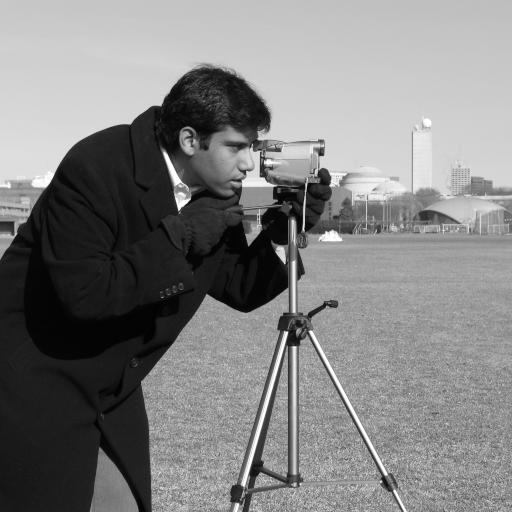
\includegraphics[width=5.0 cm]{images/originals/camera.jpg}}
		\subfigure[T\'orax 1]{
			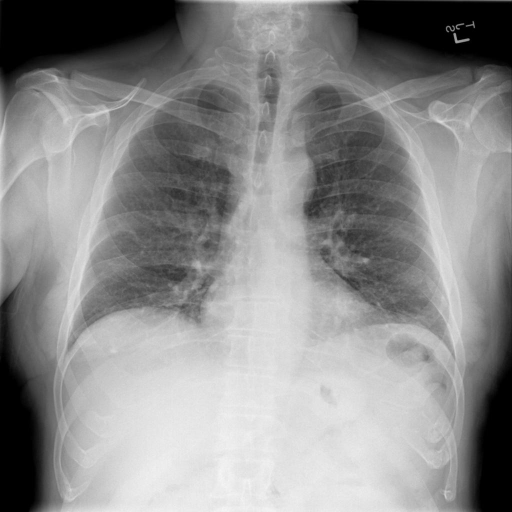
\includegraphics[width=5.0 cm]{images/originals/torax.png}}
		\caption{Im\'agenes para los experimentos de detecci\'on de bordes}
	\end{center}
\end{figure}

\begin{figure}
	\begin{center}
		\subfigure[Lineal $C_p=4.69$]{
			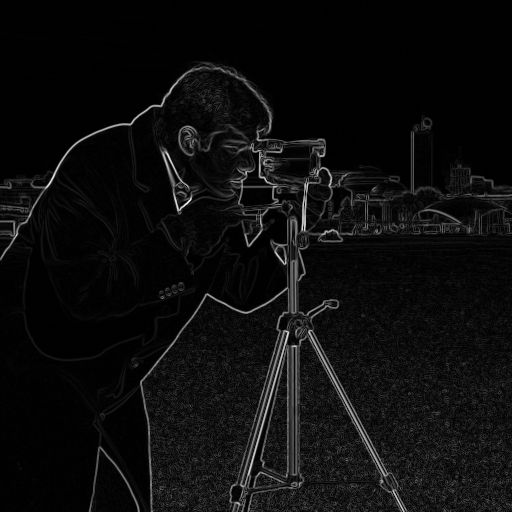
\includegraphics[width=4.0 cm]{images/scharr/camera/sla.png}}
		\subfigure[LIP $C_p=7.43$]{
			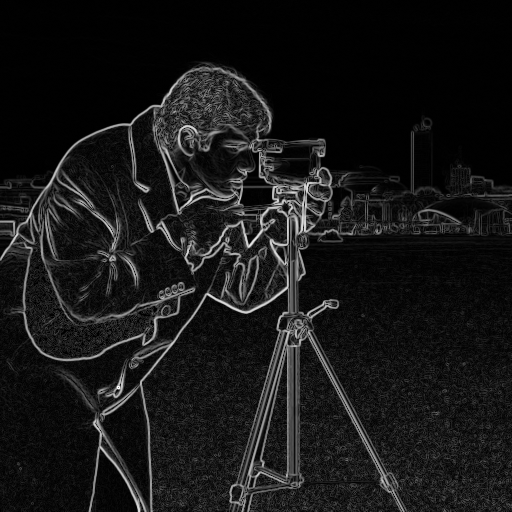
\includegraphics[width=4.0 cm]{images/scharr/camera/sja.png}}
		\subfigure[HLIP $C_p=8.05$]{
			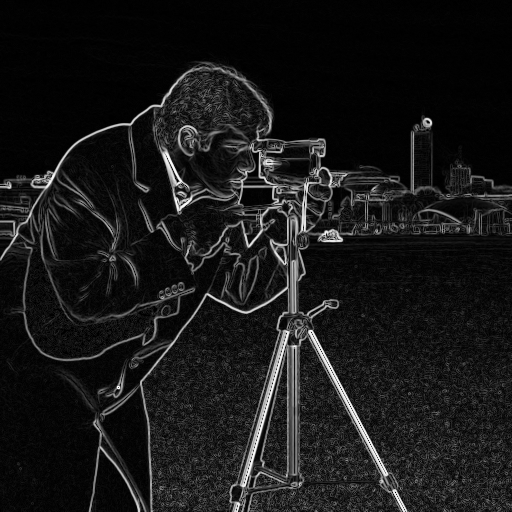
\includegraphics[width=4.0 cm]{images/scharr/camera/sha.png}}
		\subfigure[PSLIP $C_p=9.41$]{
			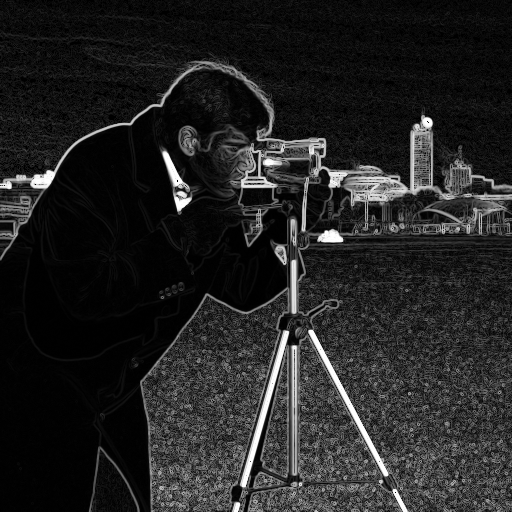
\includegraphics[width=4.0 cm]{images/scharr/camera/spsa.png}}
		\subfigure[SLIP $C_p=6.26$]{
			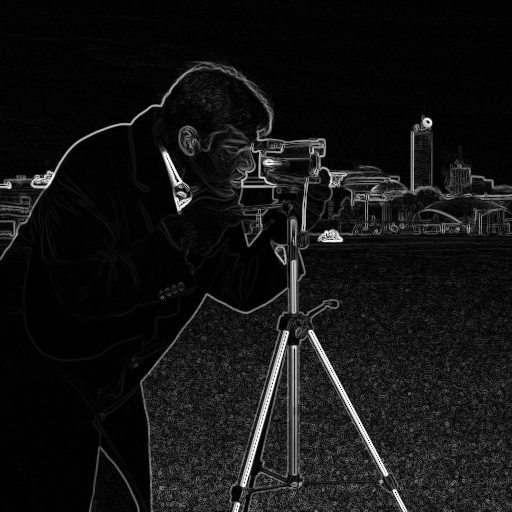
\includegraphics[width=4.0 cm]{images/scharr/camera/ssa.png}}
		\subfigure[PLIP $C_p=7.43$]{
			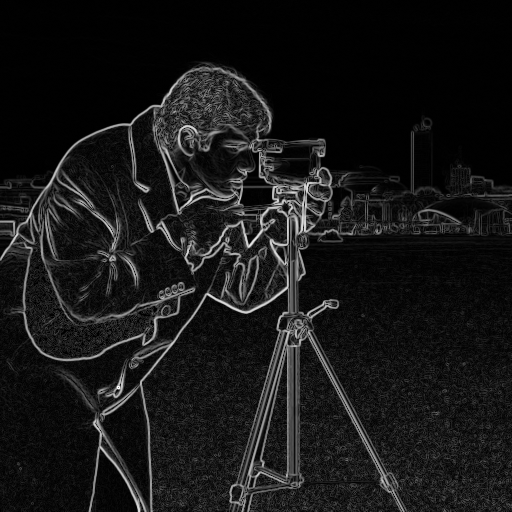
\includegraphics[width=4.0 cm]{images/scharr/camera/spa.png}}
		\subfigure[PPSLIP $C_p=9.41$]{
			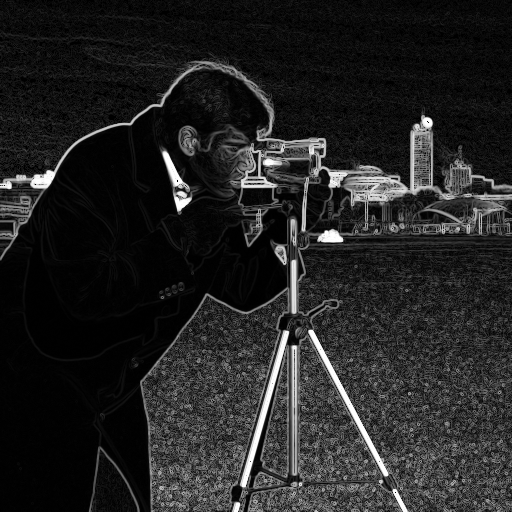
\includegraphics[width=4.0 cm]{images/scharr/camera/sppsa.png}}
		\caption{Filtro de Scharr aplicado a la imagen C\'amara con los diferentes modelos}
	\end{center}
\end{figure}

\begin{figure}
	\begin{center}
		\subfigure[Lineal $C_p=2.89$]{
			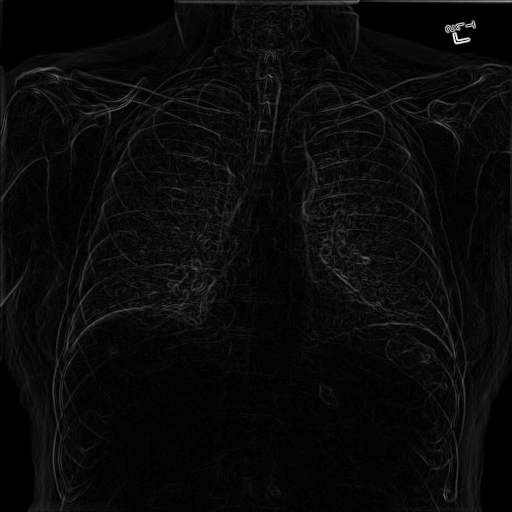
\includegraphics[width=4.0 cm]{images/scharr/torax/slb.png}}
		\subfigure[LIP $C_p=3.66$]{
			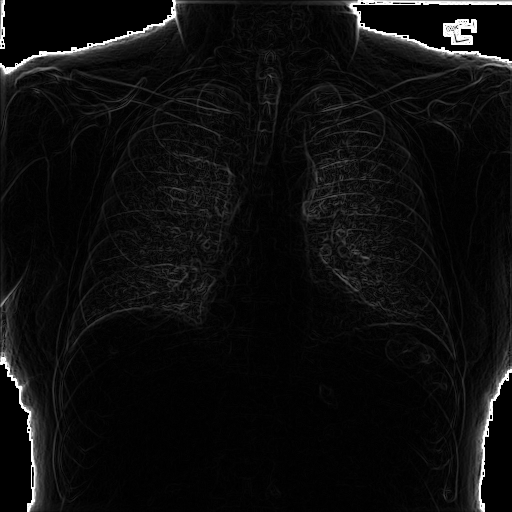
\includegraphics[width=4.0 cm]{images/scharr/torax/sjb.png}}
		\subfigure[HLIP $C_p=4.40$]{
			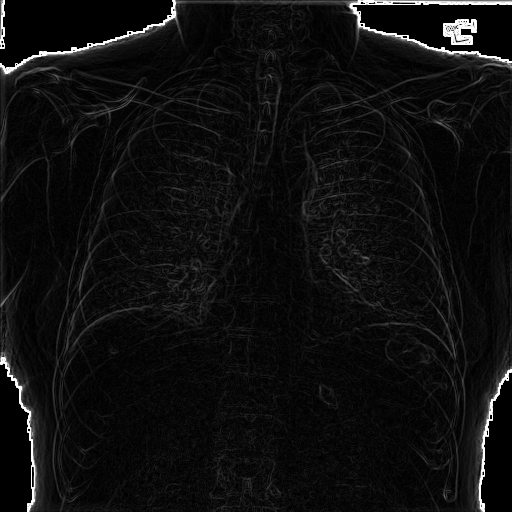
\includegraphics[width=4.0 cm]{images/scharr/torax/shb.png}}
		\subfigure[PSLIP $C_p=9.73$]{
			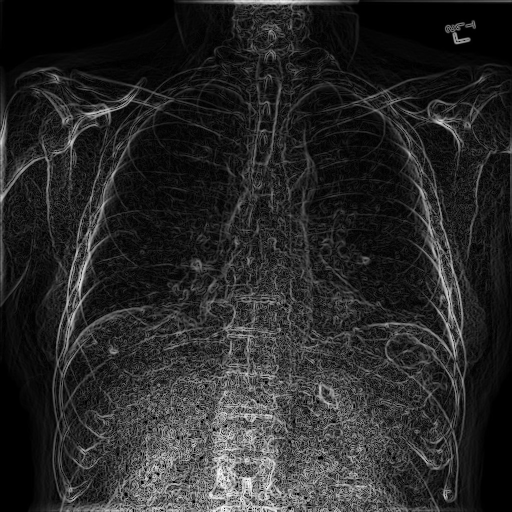
\includegraphics[width=4.0 cm]{images/scharr/torax/spsb.png}}
		\subfigure[SLIP $C_p=6.85$]{
			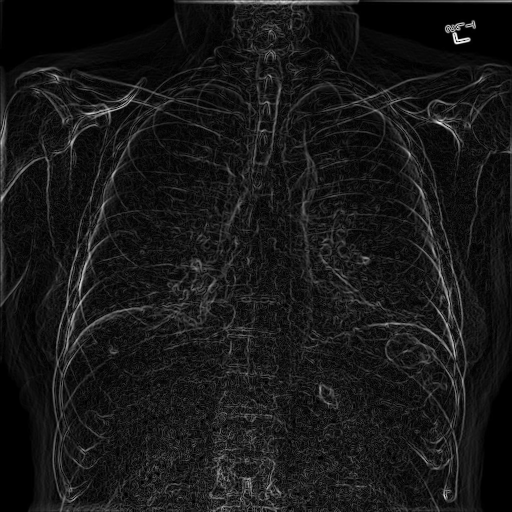
\includegraphics[width=4.0 cm]{images/scharr/torax/ssb.png}}
		\subfigure[PLIP $C_p=3.66$]{
			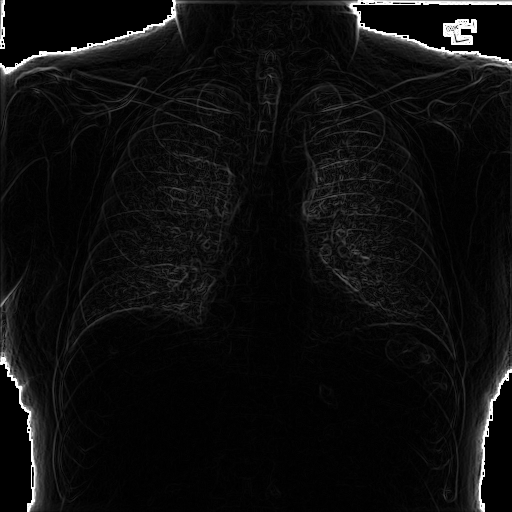
\includegraphics[width=4.0 cm]{images/scharr/torax/spb.png}}
		\subfigure[PPSLIP $C_p=9.73$]{
			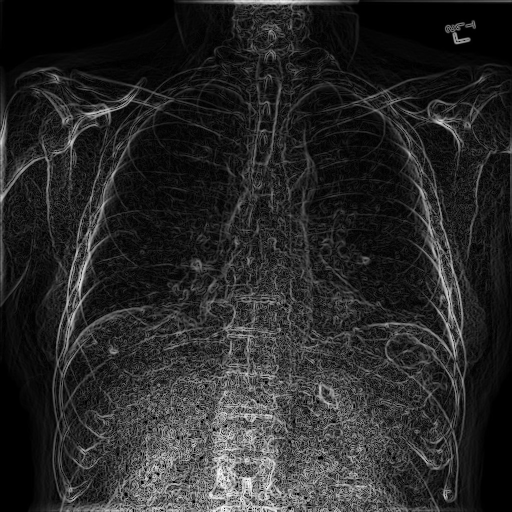
\includegraphics[width=4.0 cm]{images/scharr/torax/sppsb.png}}
		\caption{Filtro de Scharr aplicado a la imagen T\'orax con los diferentes modelos 1}
	\end{center}
\end{figure} 

Como se puede ver en la Fig 3.8 el modelo lineal se queda bastante rezagado con respecto a los modelos logar\'itmicos en cuanto al contraste promedio $C_p$. Esto adem\'as lo evidencia que el modelo PLIP arroj\'o un resultado similar al modelo LIP. Otro detalle es que el modelo LIP detect\'o mejor los bordes en las tonalidades m\'as oscuras, mientras que el SLIP hizo lo propio para las tonalidades m\'as claras. Clara evidencia esto de a que niveles de gris son m\'as sensibles estos dos modelos. El modelo SLIP por su parte dio un resultado m\'as balanceado arrojando un valor de $C_p$ superior a los anteriores. Sin dudas el mejor resultado se obtuvo utilizando el modelo PSLIP, lo cual se puede comprobar visualmente y mediante el valor de $C_p$, esto gracias a la gran sensibilidad de este modelo a las tonalidades m\'as claras, lo cual era de esperarse al ver la curva de dicho isomorfismo. Dada que este fue el mejor resultado, por ende el modelo PPSLIP coincide con este. Aunque el PSLIP da muy buenos resultados se puede apreciar que para las tonalidades oscuras es superado por el LIP y el HLIP, una soluci\'on a esto pudiera ser invertir la escala de grises tal como se hace en el modelo LIP, aunque se perder\'ia la gran sensibilidad a tonalidades claras. Adem\'as se debe tener cuidado ya que su alta sensibilidad lo hace tambi\'en muy sensible al ruido.

En este experimento los par\'ametros a estimar fueron $\lambda(M)$ para PLIP y PPSLIP, adem\'as de $\mu(M)$ en el caso de PPSLIP. La selecci\'on de estos par\'ametros se hizo de una forma similar a la explicada para la suma, lo que obviamente aplicada a la funci\'on del isomorfismo.

Un uso muy pr\'actico de los filtros para la detecci\'on de bordes es im\'agenes m\'edicas. Como se dijo anteriormente un ejemplo de estos se puede apreciar en la Fig 3.9 utilizando los diferentes modelos. En este ejemplo se puede apreciar visualmente como todos los modelos logar\'itmicos superan al modelo lineal, lo cual es confirmado por el valor de $C_p$. Al ser una imagen donde predominan las tonalidades claras es l\'ogico que el modelo LIP arroje los peores resultados, seguido del modelo HLIP. El SLIP arroja un muy buen resultado, pero es superado en gran medida por el modelo PSLIP (y por ende el PPSLIP), dando una imagen muy detallada y de muy buena calidad. El valor de $C_p$ confirma esta apreciaci\'on visual.

\subsection{Unsharp Masking}

Los pr\'oximos experimentos que se presentan a continuaci\'on es la aplicaci\'on del algoritmo de \textit{Unsharp Masking} utilizando los diferentes modelos. Para la realizaci\'on de los mismos, al igual que en los casos anteriores, se pueden utilizar las funciones implementadas para este cometido y que fueron descritas en la secci\'on \textbf{Detalles de implementaci\'on} o hacerlo manualmente siguiendo el procedimiento descrito. Las im\'agenes utilizadas en estos experimentos ser\'an las mismas ya usadas anteriormente: C\'amara y T\'orax 1. Los resultados de estos experimentos se pueden apreciar en las Fig 3.10 y y 3.11 respectivamente.

\begin{figure}
	\begin{center}
		\subfigure[Original $C_p=5.00$]{
			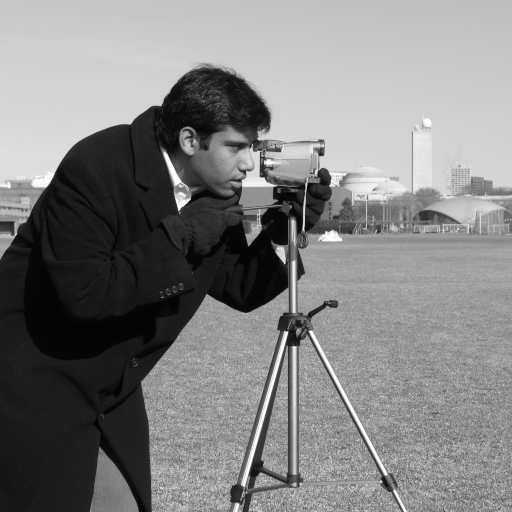
\includegraphics[width=4.0 cm]{images/unsharp_masking/camera/camera.png}}
		\subfigure[Lineal $C_p=4.13$]{
			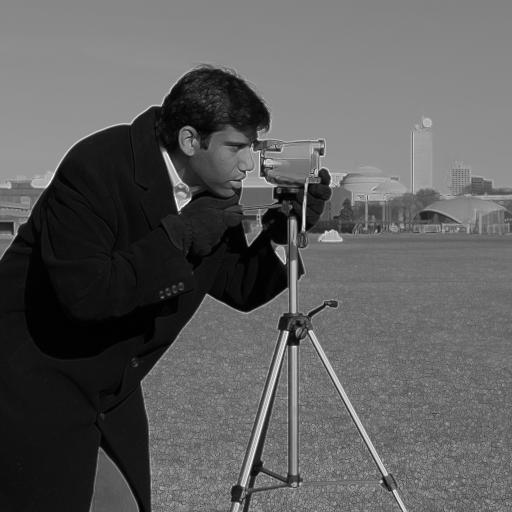
\includegraphics[width=4.0 cm]{images/unsharp_masking/camera/la_sla.png}}
		\subfigure[LIP $C_p=5.14$]{
			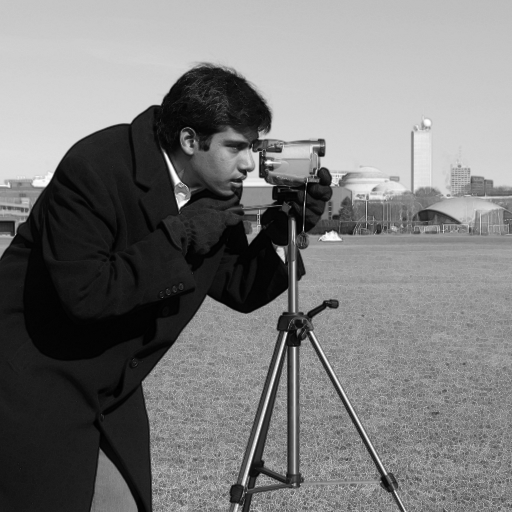
\includegraphics[width=4.0 cm]{images/unsharp_masking/camera/ja_sja.png}}
		\subfigure[HLIP+ $C_p=5.66$]{
			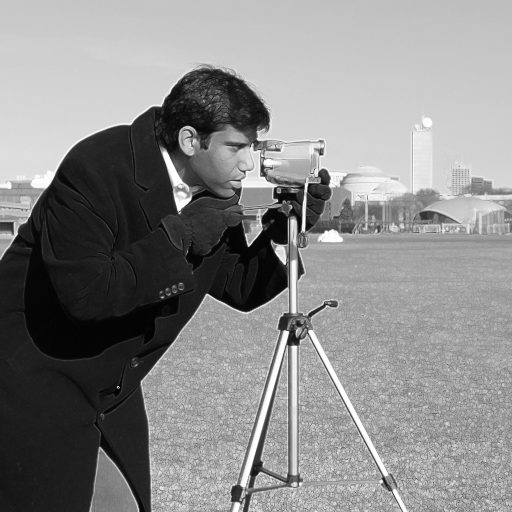
\includegraphics[width=4.0 cm]{images/unsharp_masking/camera/ha_sha+.png}}
		\subfigure[HLIP- $C_p=5.73$]{
			\includegraphics[width=4.0 cm]{images/unsharp_masking/camera/ha_sha-.png}}
		\subfigure[PSLIP $C_p=4.84$]{
			\includegraphics[width=4.0 cm]{images/unsharp_masking/camera/psa_spsa.png}}
		\subfigure[SLIP $C_p=5.16$]{
			\includegraphics[width=4.0 cm]{images/unsharp_masking/camera/sa_ssa.png}}
		\subfigure[PLIP $C_p=5.14$]{
			\includegraphics[width=4.0 cm]{images/unsharp_masking/camera/pa_spa.png}}
		\subfigure[PPSLIP $C_p=5.80$]{
			\includegraphics[width=4.0 cm]{images/unsharp_masking/camera/ppsa_sppsa.png}}
		\caption{Unsharp masking aplicado a la imagen C\'amara con los diferentes modelos}
	\end{center}
\end{figure}

\begin{figure}
	\begin{center}
		\subfigure[Original $C_p=2.26$]{
			\includegraphics[width=4.0 cm]{images/unsharp_masking/torax/CXR7_IM-2263-1001.png}}
		\subfigure[Lineal $C_p=2.60$]{
			\includegraphics[width=4.0 cm]{images/unsharp_masking/torax/lb_slb.png}}
		\subfigure[LIP $C_p=2.53$]{
			\includegraphics[width=4.0 cm]{images/unsharp_masking/torax/jb_sjb.png}}
		\subfigure[HLIP+ $C_p=3.46$]{
			\includegraphics[width=4.0 cm]{images/unsharp_masking/torax/hb_shb+.png}}
		\subfigure[HLIP- $C_p=2.62$]{
			\includegraphics[width=4.0 cm]{images/unsharp_masking/torax/hb_shb-.png}}
		\subfigure[PSLIP $C_p=2.52$]{
			\includegraphics[width=4.0 cm]{images/unsharp_masking/torax/psb_spsb.png}}
		\subfigure[SLIP $C_p=2.59$]{
			\includegraphics[width=4.0 cm]{images/unsharp_masking/torax/sb_ssb.png}}
		\subfigure[PLIP $C_p=2.53$]{
			\includegraphics[width=4.0 cm]{images/unsharp_masking/torax/pb_spb.png}}
		\subfigure[PPSLIP $C_p=4.97$]{
			\includegraphics[width=4.0 cm]{images/unsharp_masking/torax/ppsb_sppsb.png}}
		\caption{Unsharp masking aplicado a la imagen T\'orax 1 con los diferentes modelos}
	\end{center}
\end{figure}

En la Fig 3.10 se puede apreciar como este algoritmo para el caso lineal de una imagen incluso peor a la imagen original pues esta es muy oscura y los bordes no se aprecian muy bien definidos, lo cual tambi\'en lo confirma el valor de $C_p$. El modelo LIP da una mejor soluci\'on. Aprovech\'andose el car\'acter sim\'etrico del modelo HLIP se analizaron dos variantes de fusi\'on: la suma y la resta. Para este ejemplo se puede comprobar visualmente que la mejor imagen obtenida fue la resultante de la fusi\'on mediante la resta, lo cual tambi\'en es confirmado por el valor de $C_p$. 

El modelo PSLIP tampoco ofrece un mejor resultado, esto debido a que no se logra una buena fusi\'on entre la imagen original y la imagen de bordes, algo similar a lo que ocurri\'o en en el primer experimento de suma de im\'agenes presentado. El modelo SLIP tambi\'en da un buen resultado, con un valor de $C_p$ muy parecido al del modelo LIP. El modelo PLIP se asemej\'o a un comportamiento logar\'itmico como era de esperarse dados los resultados del modelo lineal y PLIP. Tambi\'en se puede apreciar como el modelo PPSLIP resuelve el problema del modelo PSLIP, arrojando una imagen de mayor calidad, siendo esta la de mejor valor de $C_p$. V\'alido se\~nalar que esta \'ultima resalta mucho los bordes por lo que quiz\'as ser\'ia mejor utilizar otro modelo o utilizar par\'ametros que den una imagen m\'as suave seg\'un la situaci\'on.

Aqu\'i tambi\'en es bueno aclarar que para los modelos parametrizados se utiliz\'o como par\'ametro para la funci\'on del isomorfismo el par\'ametro que di\'o el mejor resultado en la detecci\'on de bordes para cada modelo. Dado esto entonces, lo que se hizo fue buscar los mejores par\'ametros que dieran el mejor resultado para la fusi\'on.

En la Fig 3.11 si bien todos los modelos resaltan en alguna medida los bordes y mejoran el valor de contraste promedio con respecto a la imagen original, los resultados no se diferencian mucho unos de otros, salvo los casos del modelo HLIP con fusi\'on por suma y del PPSLIP. Este \'ultimo arroja una imagen mucho m\'as detallada y por ende de mayor calidad que el resto de los modelos, algo que se puede comprobar tanto visualmente como por el valor de $C_p$. Esto confirma una vez m\'as la eficacia y utilidad del modelo propuesto.

\subsection{Transformaci\'on af\'in}

A continuaci\'on se presentan los experimentos basados en la modificaci\'on del histograma. Espec\'ificamente se analizar\'a la ecualizaci\'on del histograma que  que ``extiende los valores de intensidad más frecuentes'' y ya viene implementada el m\'odulo \verb|skimage.exposure|~\cite{histogram_equalization}. Aunque si bien la ecualización del histograma tiene la ventaja de que no requiere parámetros, a veces produce imágenes de aspecto poco natural. Los otros algoritmos analizados ser\'a el de transformaci\'on af\'in utilizando los modelos HLIP y SLIP. Para el caso del modelo SLIP antes de aplicar la transformaci\'on af\'in primero se extiende la imagen por todo el rango de valores $(-M,M)$, utilizando la transformaci\'on lineal $2\cdot(f-M/2)$ donde $f$ es una imagen. Esta transformaci\'on se hizo para aprovechar todo el rango de valores del modelo SLIP y obtener mejores resultados pero no es algo inherente al modelo. Esta es una de las ventajas que tiene usar los modelos definidos desde un punto de vista de matem\'atico. Las im\'agenes utilizadas en los experimentos que se presentan son im\'agenes de bajo contraste: Luna y T\'orax 2. Los experimentos sobre estas im\'agenes se pueden observar en las Fig 3.12 y Fig 3.13 respectivamente.

\begin{figure}
	\begin{center}
		\subfigure[Original $C_p=1.30$]{
			\includegraphics[width=4.3 cm]{images/he/moon/imgs/moon.png}}
		\subfigure[Original Histograma]{
			\includegraphics[width=6.0 cm]{images/he/moon/hists/oa_hist.png}}
		\subfigure[Ecualizada $C_p=10.86$]{
			\includegraphics[width=4.3 cm]{images/he/moon/imgs/limg_eq_a.png}}
		\subfigure[Ecualizada Histograma]{
			\includegraphics[width=6.0 cm]{images/he/moon/hists/leqa_hist.png}}
		\subfigure[Transformaci\'on HLIP $C_p=5.35$]{
			\includegraphics[width=4.33 cm]{images/he/moon/imgs/himg_eq_a.png}}
		\subfigure[Transformaci\'on HLIP Histograma]{
			\includegraphics[width=6.0 cm]{images/he/moon/hists/hata_hist.png}}
		\subfigure[Transformaci\'on SLIP $C_p=5.07$]{
			\includegraphics[width=4.3 cm]{images/he/moon/imgs/simg_eq_a.png}}
		\subfigure[Transformaci\'on SLIP Histograma]{
			\includegraphics[width=6.0 cm]{images/he/moon/hists/sata_hist.png}}
		\caption{Diferentes t\'ecnicas de ecualizaci\'on del histograma de la imagen Luna}
	\end{center}
\end{figure}

\begin{figure}
	\begin{center}
		\subfigure[Original $C_p=1.05$]{
			\includegraphics[width=5.0 cm]{images/he/torax/imgs/torax.png}}
		\subfigure[Original Histograma]{
			\includegraphics[width=5.5 cm]{images/he/torax/hists/ob_hist.png}}
		\subfigure[Ecualizada $C_p=2.82$]{
			\includegraphics[width=5.0 cm]{images/he/torax/imgs/limg_eq_b.png}}
		\subfigure[Ecualizada Histograma]{
			\includegraphics[width=5.5 cm]{images/he/torax/hists/leqb_hist.png}}
		\subfigure[Transformaci\'on HLIP $C_p=2.36$]{
			\includegraphics[width=5.0 cm]{images/he/torax/imgs/himg_eq_b.png}}
		\subfigure[Transformaci\'on HLIP Histograma]{
			\includegraphics[width=5.5 cm]{images/he/torax/hists/hatb_hist.png}}
		\subfigure[Transformaci\'on SLIP $C_p=2.19$]{
			\includegraphics[width=5.0 cm]{images/he/torax/imgs/simg_eq_b.png}}
		\subfigure[Transformaci\'on SLIP Histograma]{
			\includegraphics[width=5.5 cm]{images/he/torax/hists/satb_hist.png}}
		\caption{Diferentes t\'ecnicas de ecualizaci\'on del histograma de la imagen T\'orax 2}
	\end{center}
\end{figure}

En la Fig 3.12 se puede apreciar de forma visual como la imagen Luna es una imagen con muy poco contraste. Su histograma y el valor de $C_p$ confirman esta apreciaci\'on. Luego se ve como aplicando una ecualizaci\'on del histograma la imagen mejora su contraste, pero quiz\'as se pueda considerar como una imagen poco natural, aunque esto ya es una cuesti\'on subjetiva. Aqu\'i es bueno recalcar que a pesar de que el valor de contraste promedio ($C_p$) en los experimentos realizados ha mostrado resultados consecuentes con la calidad de la imagen, esto no quiere decir que la calidad de una imagen dependa exclusivamente de su contraste, de hecho no lo hace. Para determinar la calidad de una imagen se pueden utilizar otras medidas objetivas pero al final lo m\'as importante es la calidad que pueda percibir un usuario al mirar la imagen, lo cual es una medida subjetiva. Bajo este criterio es posible que prefieran transformaciones m\'as suaves como las que arrojan las transformaciones afines en los modelos HLIP y SLIP. Para ambos modelos se obtiene un buen valor de contraste y la imagen obtenida se percibe bastante natural.

En la Fig 3.13 observamos que la imagen del t\'orax captada por el equipo que la tomo tuvo igual un muy bajo contraste; y como los diferentes algoritmos dan resultados que mejoran tanto la calidad visual percibida como el valor de contraste promedio. Esto tambi\'en se ve reflejado en como se expanden los valores de intensidad por el histograma.

Al fijarse en los histogramas de ambas figuras se puede comprobar como la ecualizaci\'on del histograma es la transformaci\'on m\'as fuerte, la transformaci\'on af\'in utilizando el modelo HLIP  es muy parecida a la transformaci\'on af\'in utilizando el modelo SLIP, aunque la del HLIP es un poco m\'as fuerte. Esto adem\'as es confirmado por el valor de $C_p$ en ambos casos.

Una algoritmo muy bueno e interesante es la Ecualización Adaptativa Limitada por Contraste del Histograma (CLAHE) que tambi\'en aparece implementada en \verb|skimage.exposure|~\cite{module_exposure}. Este es un algoritmo para la mejora del contraste local, que utiliza histogramas calculados sobre diferentes regiones de mosaico de la imagen. Por lo tanto, los detalles locales se pueden mejorar incluso en regiones que son más oscuras o más claras que la mayoría de la imagen. Ser\'ia interesante implementar un algoritmo que siguiera esta idea de calcular los histogramas de manera local pero utilizando el algoritmo de transformaci\'on af\'in con los diferentes modelos.